\documentclass[12pt,letterpaper,oneside,reqno]{amsart}
\usepackage{amsfonts}
\usepackage{amsmath}
\usepackage{amssymb}
\usepackage{amsthm}
\usepackage{float}
\usepackage{mathrsfs}
\usepackage{colonequals}
\usepackage[font=small,labelfont=bf]{caption}
\usepackage[left=1in,right=1in,bottom=1in,top=1in]{geometry}
\usepackage[pdfpagelabels,hyperindex,colorlinks=true,linkcolor=blue,urlcolor=magenta,citecolor=green]{hyperref}
\usepackage{graphicx}
\linespread{1.7}
\emergencystretch=1em
\usepackage{array}
\usepackage{etoolbox}
\apptocmd{\sloppy}{\hbadness 10000\relax}{}{}
\raggedbottom

\newtheorem{theorem}{Theorem}[section]
\newtheorem{corollary}[theorem]{Corollary}
\newtheorem{lemma}[theorem]{Lemma}
\newtheorem{example}[theorem]{Example}
\newtheorem{conjecture}[theorem]{Conjecture}
\newtheorem{definition}[theorem]{Definition}

\numberwithin{equation}{section}
\pdfminorversion=7

%--------Meta Data: Fill in your info------
\title[RSA Encryption: Behind the scenes]{RSA Encryption: Behind the scenes}
\author[Petro Kolosov]{Petro Kolosov}
\address{Software Developer, DevOps Engineer}
\email{kolosovp94@gmail.com}
\urladdr{https://kolosovpetro.github.io}
\subjclass[2010]{94A60, 11T71}
\keywords{
    RSA encryption,
    Rivest-Shamir-Adleman,
    Asymmetric encryption,
    Symmetric encryption,
    Public key cryptography,
    Private key cryptography,
    Diffie-Hellman key exchange,
    One-way functions,
    Cryptographic protocols,
    Public and private keys,
    Key exchange problem,
    Encryption history,
    Cryptographic algorithms,
}
\date{\today}
\hypersetup{
    pdftitle={RSA Encryption: Behind the scenes},
    pdfsubject={
        RSA encryption,
        Rivest-Shamir-Adleman,
        Clifford Cocks,
        Asymmetric encryption,
        Symmetric encryption,
        Public key cryptography,
        Private key cryptography,
        Diffie-Hellman key exchange,
        One-way functions,
        Cryptographic protocols,
        Secure communication,
        Public and private keys,
        Key exchange problem,
        GCHQ (Government Communications Headquarters),
        Encryption history,
        Number theory in cryptography,
        Digital security,
        Opened lock analogy,
        Cryptographic algorithms,
        RSA patent expiration
    },
    pdfauthor={Petro Kolosov},
    pdfkeywords={
        RSA encryption,
        Rivest-Shamir-Adleman,
        Clifford Cocks,
        Asymmetric encryption,
        Symmetric encryption,
        Public key cryptography,
        Private key cryptography,
        Diffie-Hellman key exchange,
        One-way functions,
        Cryptographic protocols,
        Secure communication,
        Public and private keys,
        Key exchange problem,
        GCHQ (Government Communications Headquarters),
        Encryption history,
        Number theory in cryptography,
        Digital security,
        Opened lock analogy,
        Cryptographic algorithms,
        RSA patent expiration
    }
}
\begin{document}
    \begin{abstract}
        Simple explanation on the problematics and main idea behind the Rivest-Shamir-Adleman (RSA) encryption.

    \end{abstract}


    \maketitle
    \tableofcontents


    \section{RSA Encryption: General Idea}\label{sec:rsa-encryption-algorithm}
    The RSA algorithm is named after Ron \textbf{Rivest}, Adi \textbf{Shamir} and Len \textbf{Adleman}
who invented it in 1977~\cite{rivest1978method}.
The basic technique was first discovered in 1973 by Clifford Cocks~\cite{cocks1973note} of
CESG (part of the British GCHQ)
but this was a secret until 1997.
The patent taken out by RSA Labs has expired.

Historically, the process of encryption is considered to be symmetric one.
\begin{quote}
    \textbf{Symmetric encryption} -- is a type of encryption where only one secret key is
    used to both encrypt and decrypt information.
\end{quote}
It means that prior the communication the sides must conclude and share the secret key to be used in
both encryption and decryption.
Such approach is highly cost since it requires to share the defined secret keys between each actor.

\begin{figure}[H]
    \centering
    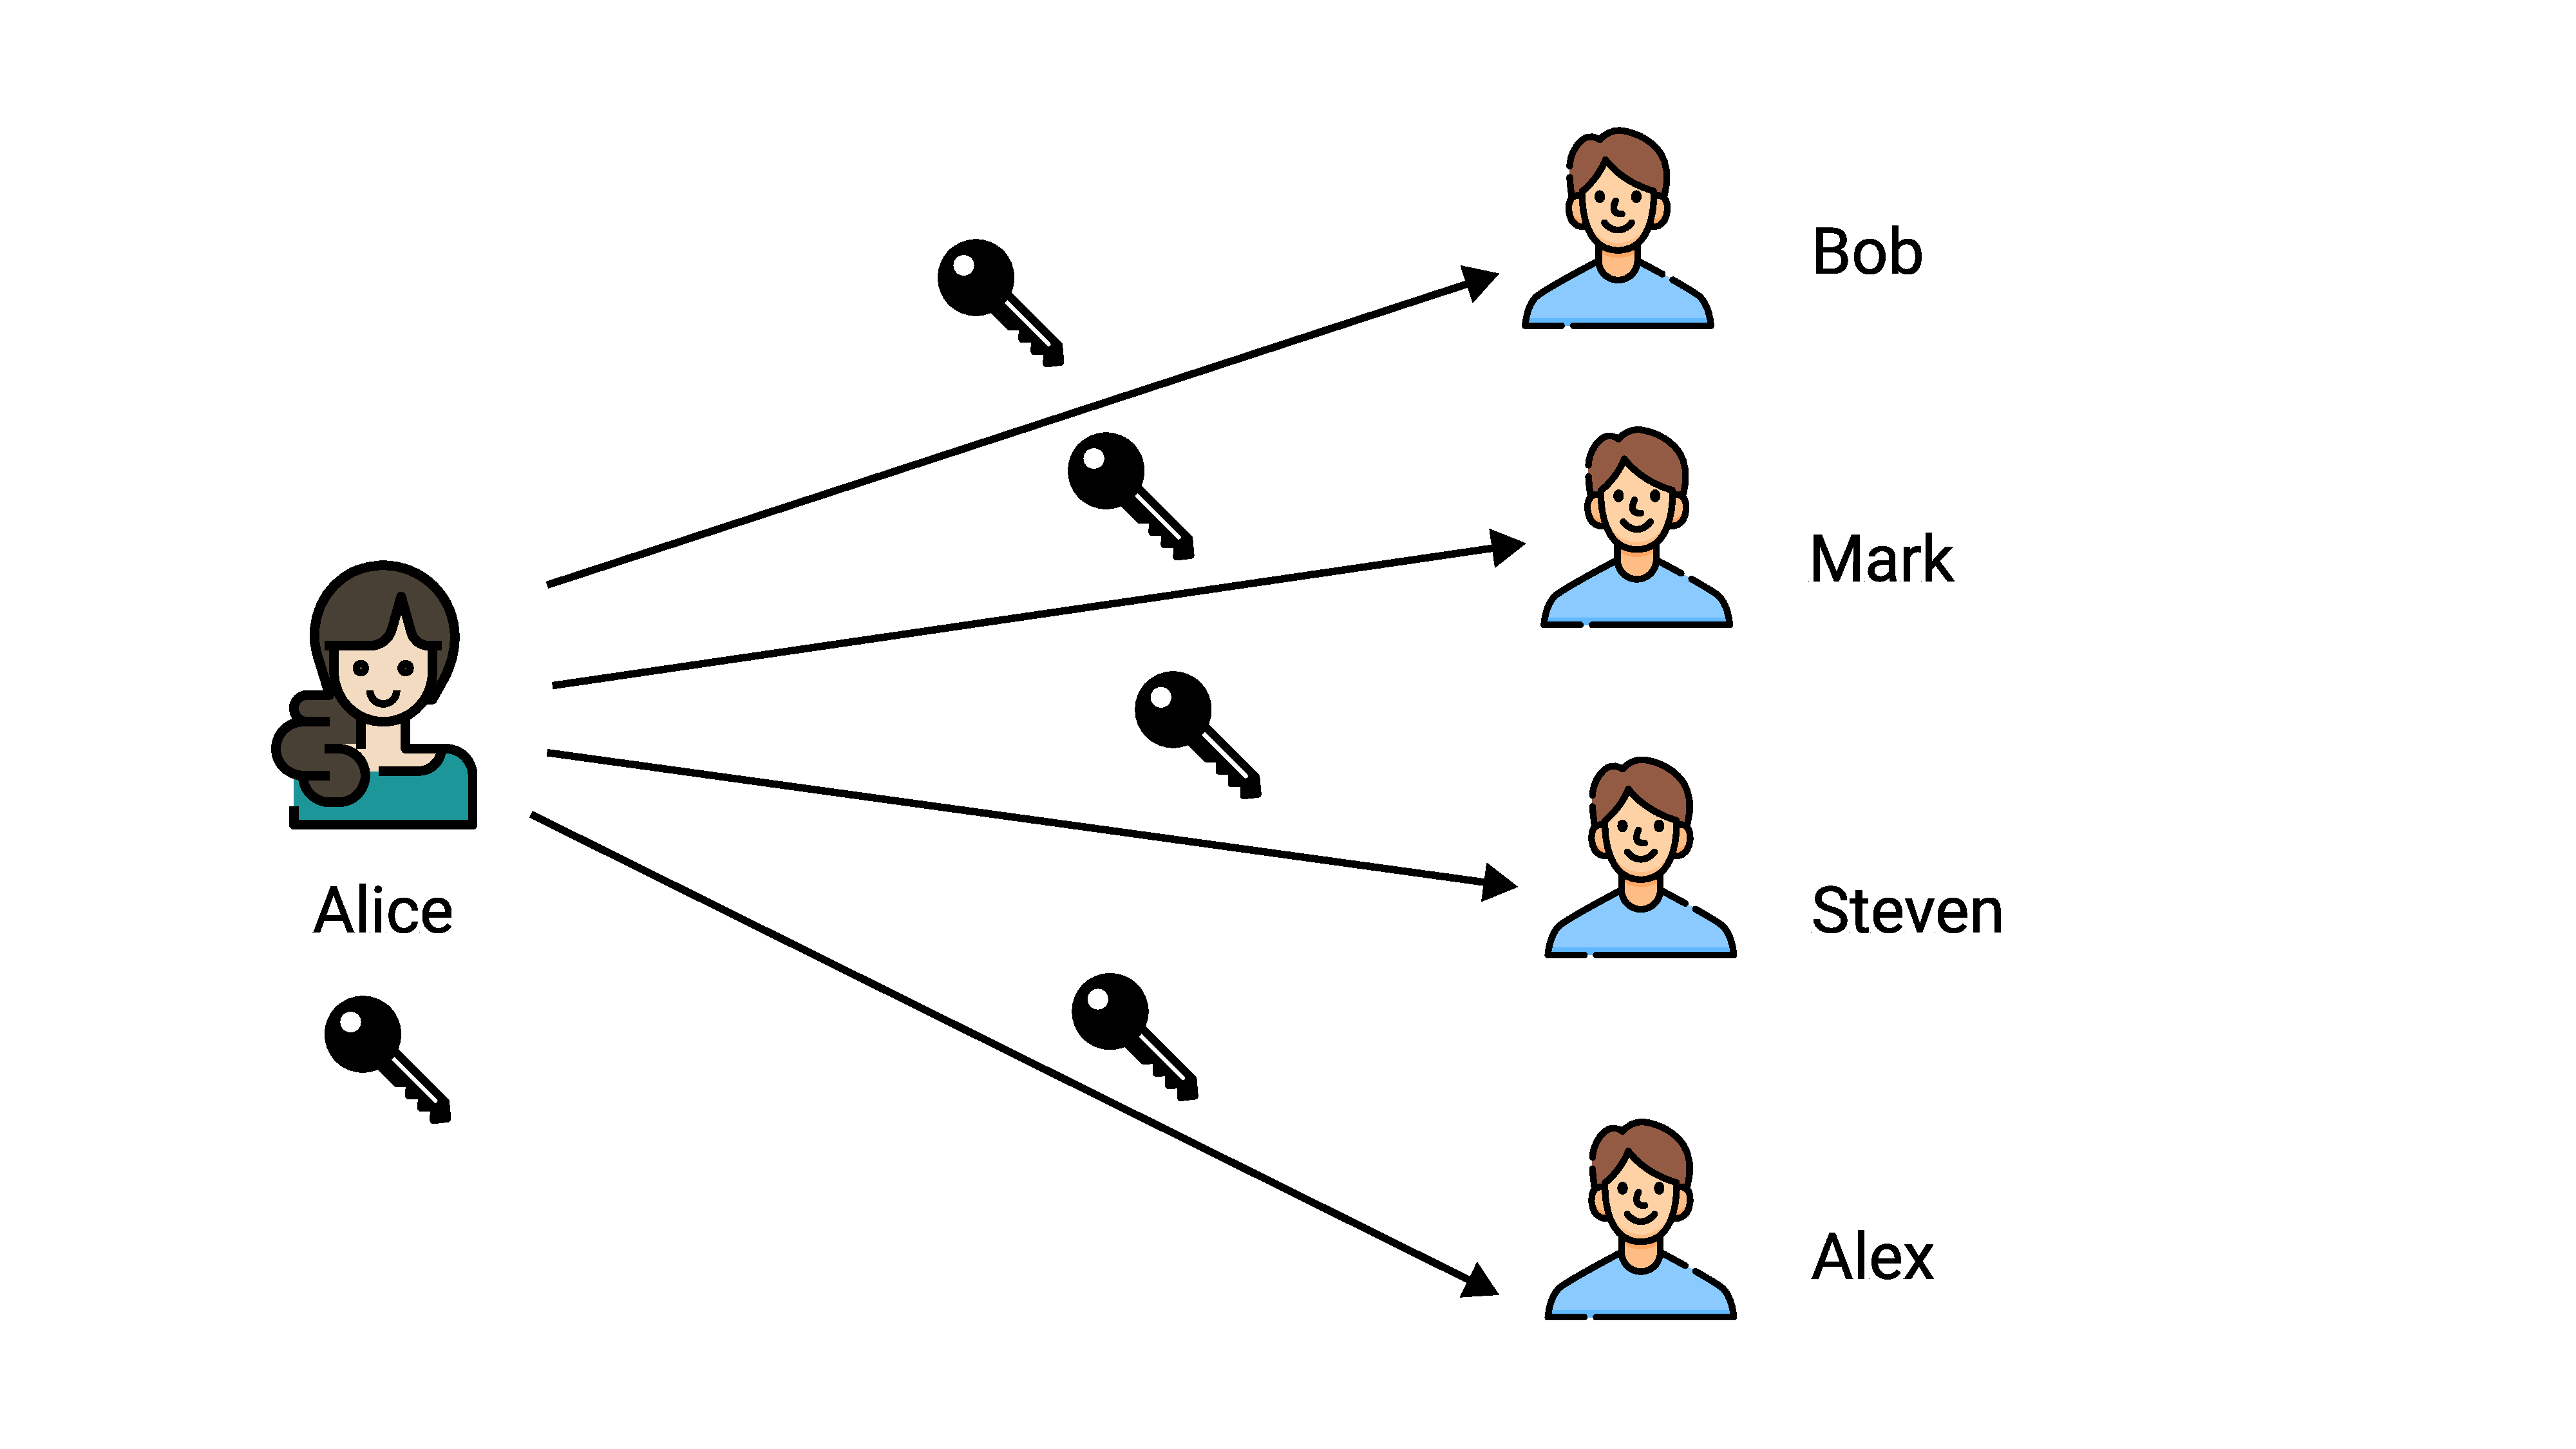
\includegraphics[width=1.15\textwidth]{./img/Symmetric_encryption}
    ~\caption{Symmetric encryption real life example.}
    \label{fig:symmetric-encryption}
\end{figure}

The problem here is that Alice, Bob, Mark, Steven and Alex must exchange the secret keys securely,
for instance by means of Diffie-Hellman key exchange.

Much more simpler is to think about secured communication channel that in terms of asymmetric encryption.
\begin{quote}
    \textbf{Asymmetric encryption} -- is an encryption such that a message is encrypted using public key and
    decrypted using private key.
\end{quote}
The real life example would be if Alice shares with all the actors not the secret key, but \textbf{opened lock}.
Still Alice keeps the key with herself, but now she doesn't worry that anyone would lose it so that key exchange must be repeated.
\begin{figure}[H]
    \centering
    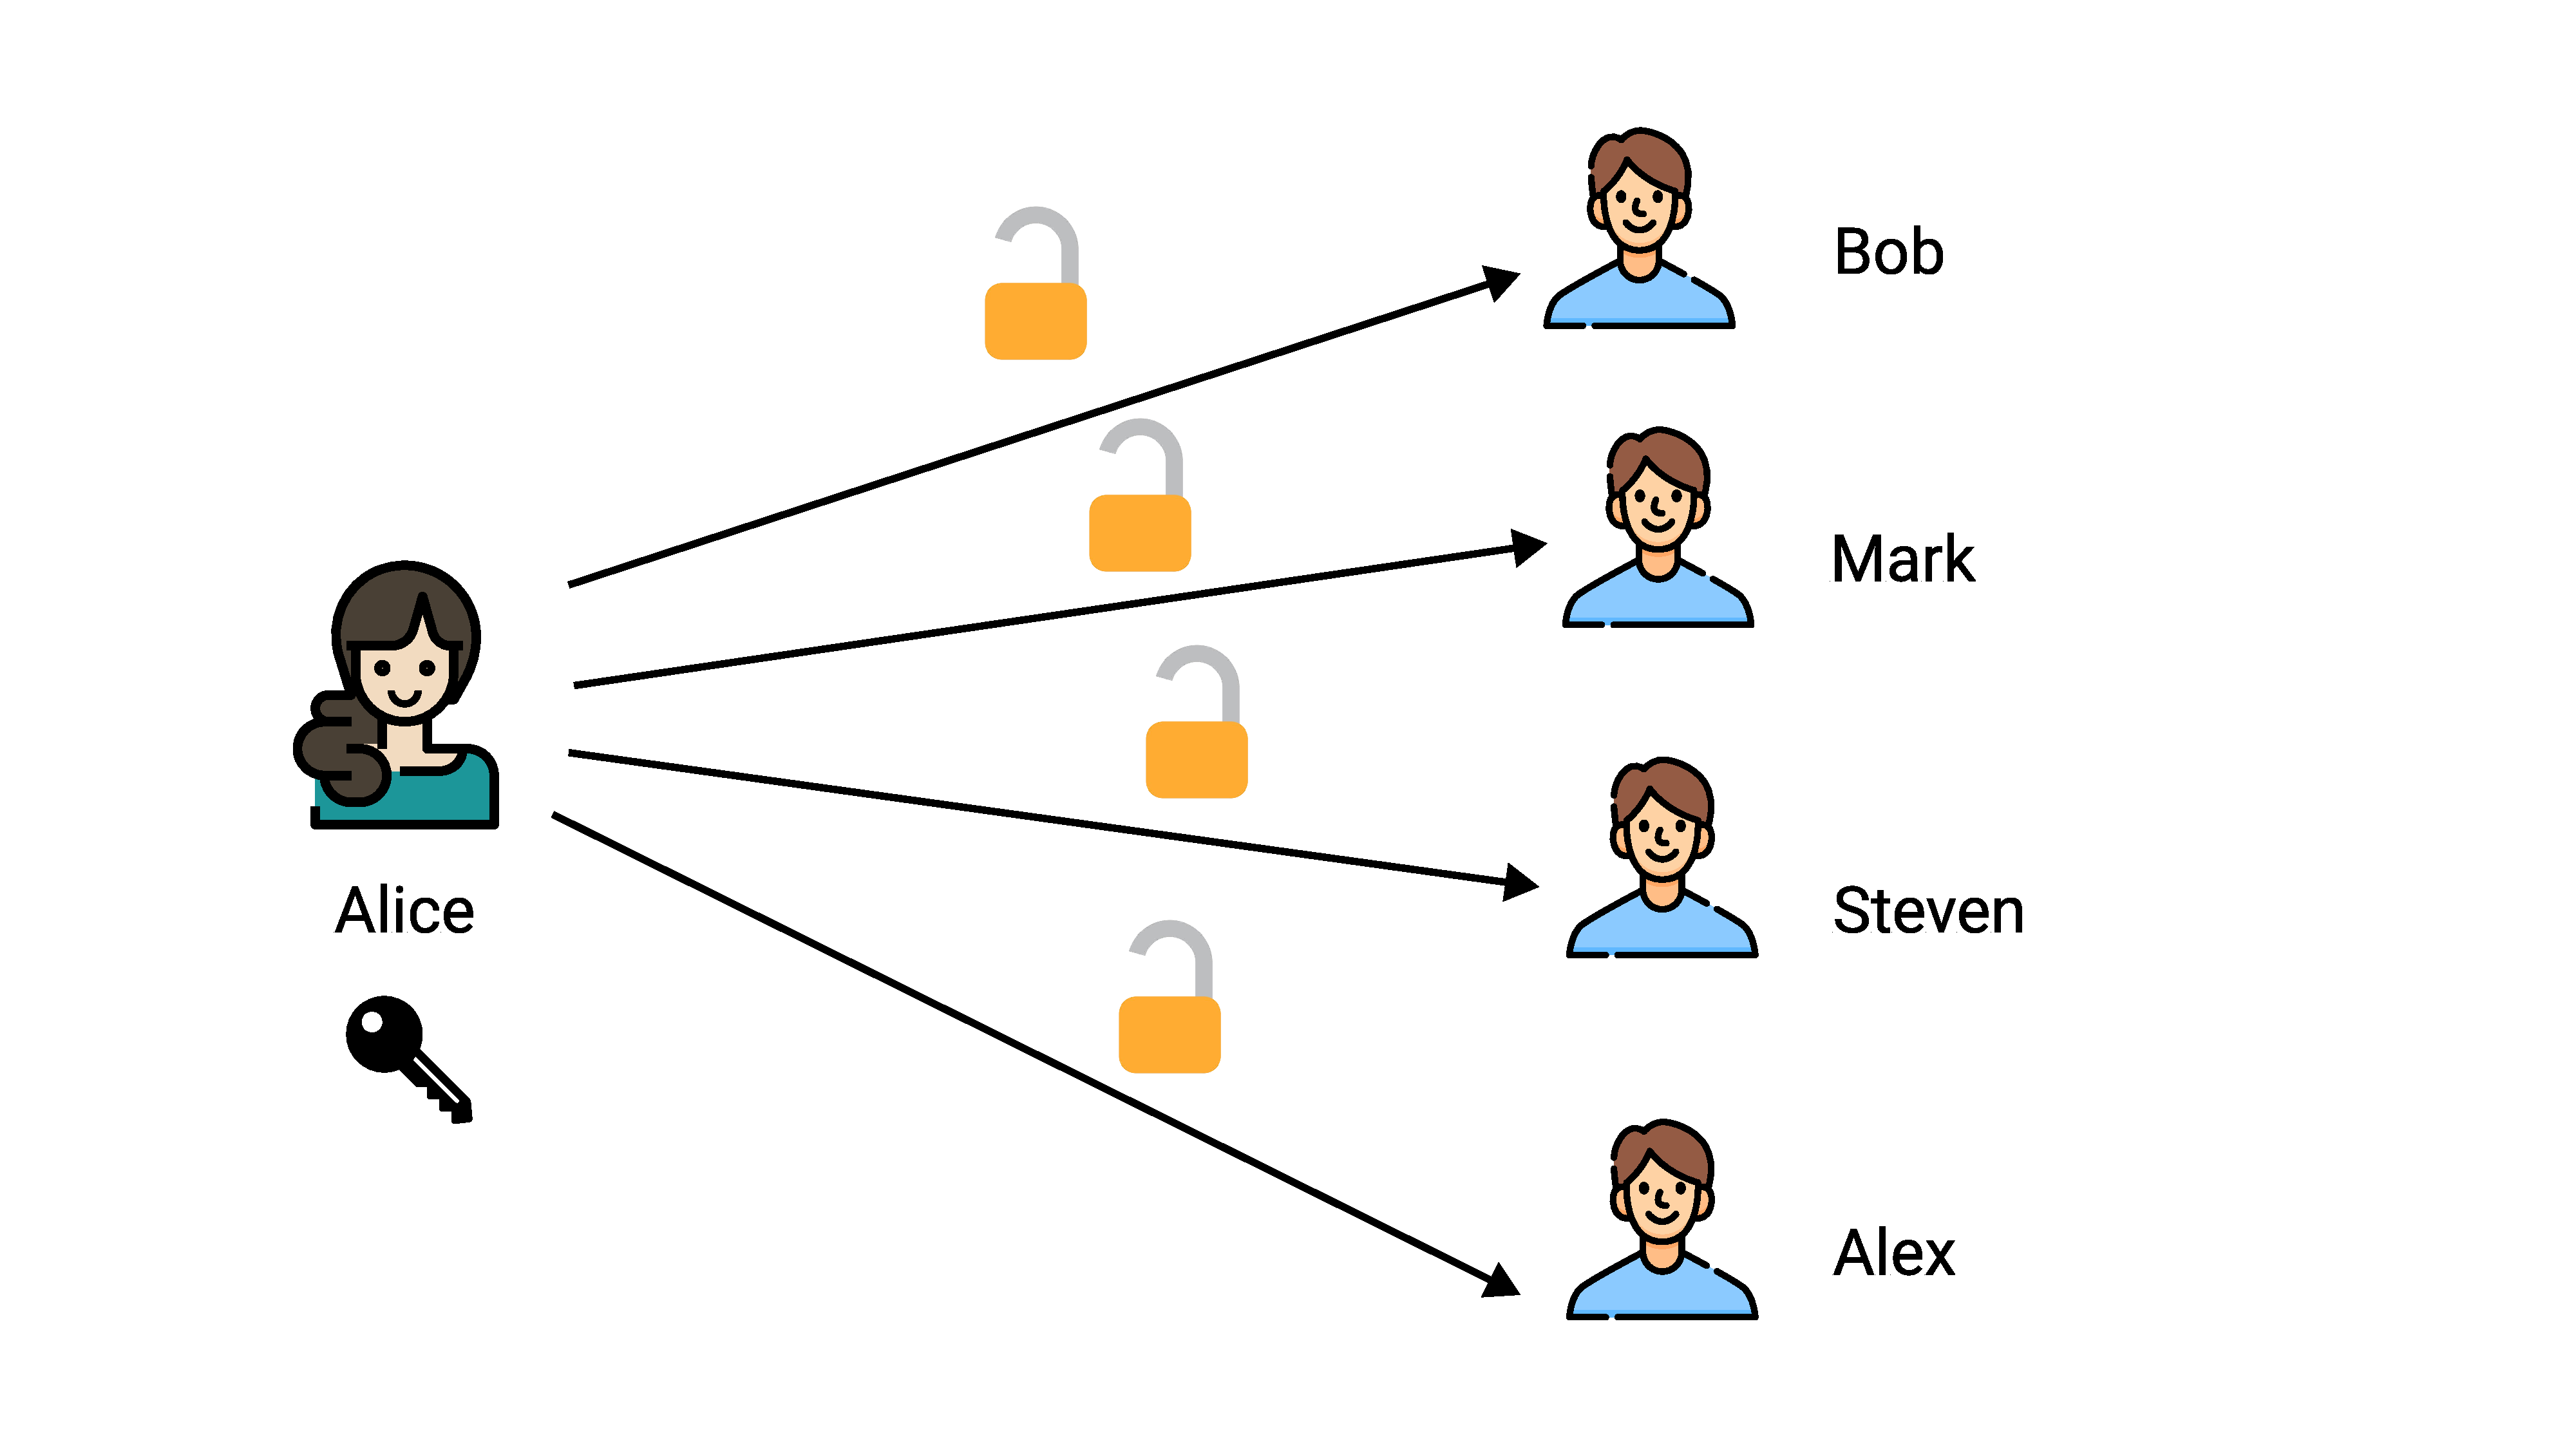
\includegraphics[width=1.15\textwidth]{./img/Asymmetric_encryption}
    ~\caption{Asymmetric encryption real life example.}\label{fig:figure2}
\end{figure}
Therefore, the Bob, Mark, Steven and Alex have received an \textbf{opened lock} or \textbf{public key} from the Alice.
Now anyone of them is able to write secret message to the Alice simply putting it to the chest closing by the lock
received from Alice so that only Alice can open it.
However, such a simple idea requires complex number theory approach.
A concept of opened lock may be interpreted in terms of one-way functions.
\begin{quote}
    \textbf{One-way function} -- is a function that is easy to compute on every input, but hard to invert given the image of
    a random input.
\end{quote}

\begin{figure}[H]
    \centering
    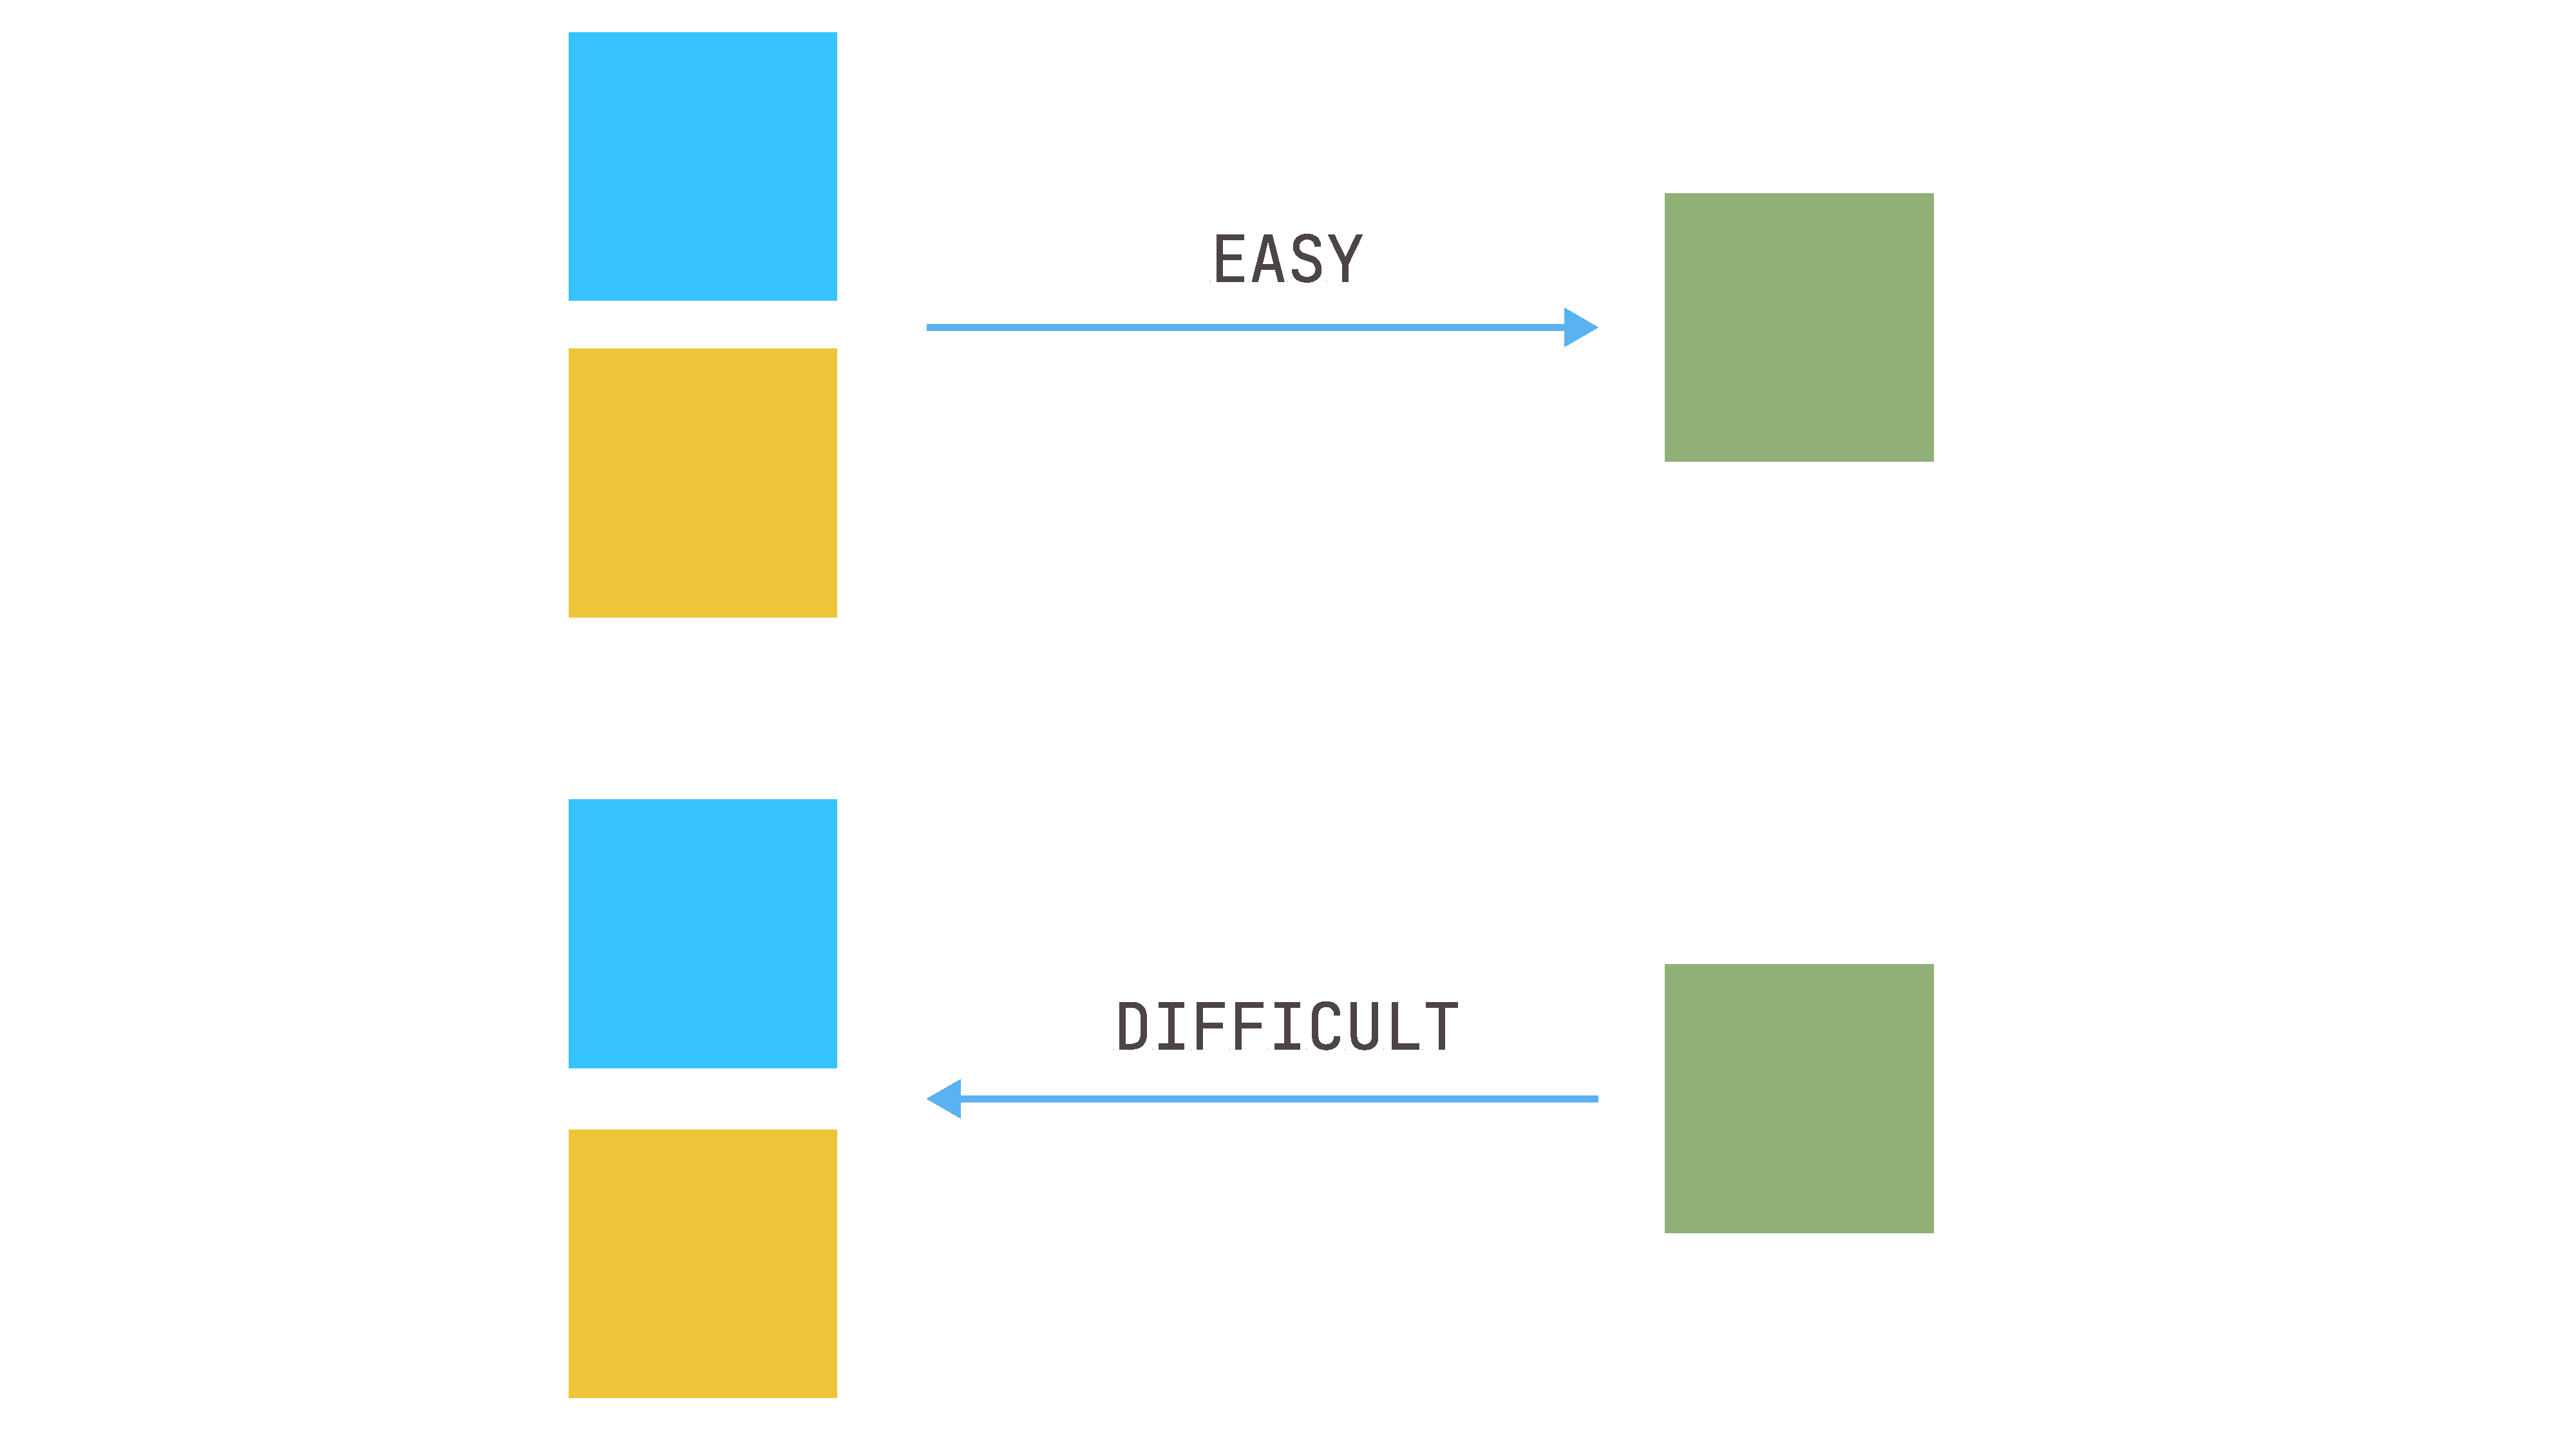
\includegraphics[width=1\textwidth]{./img/One_Way_Functions}
    ~\caption{One-way function, analogy with paints}\label{fig:figure3}
\end{figure}



    \section{Mathematics behind the RSA}\label{sec:mathematics-behind-rsa}
    For instance, the function
\begin{equation*}
    f(m) = m^e \bmod N = C, \quad (e, N) \mathrm{\; are \; public \; constants}, \quad m \; \mathrm{is \; secret}
\end{equation*}
is one-way function because it is easy to compute $C$ given $m$, but it is hard to compute $m$ given $C$.
The constants $(e, N)$ may be interpreted as an Alice's opened lock, whereas $m$ is a secret message from Bob.
Note that constants
\begin{itemize}
    \item $e$ is stands for encryption, public key
    \item $d$ is stands for decryption, private key
\end{itemize}
Now only one problem remains for the Alice -- is to define a pair of the keys $(e, d)$.
Alice knows that Bob encrypts his message $m$ as follows
\[
    m^e \bmod N = C
\]
To decrypt the message $C$ Alice must fetch a constant $d$ such that reverts the exponentiation of the
secret message $m$
\begin{eqnarray*}
    C^d = m \bmod N \\
    m^{ed} \bmod N = m \bmod N
\end{eqnarray*}
Firstly, Alice defines a public constant $N$ as a product of two large prime numbers $P, Q$
\[
    N = P \cdot Q
\]
so that it is hard to compute a factorization.

But how to fetch the secret constant $d$ to decrypt?
The Euler's totient theorem helps.
Given a number $N$ and its prime factorization $p_1^{e_1}\cdot p_2^{e_2} \cdots p_k^{e_k}$, the Euler's totient function
$\phi(N)$ is defined as
\[
    \phi(N) = (p_1^{e_1} - p_1^{e_1 - 1}) \cdot (p_2^{e_2} - p_2^{e_2 - 1}) \cdots (p_k^{e_k} - p_k^{e_k - 1})
\]
In particular, for the positive number $N$ such that its factorization is $p1 \cdot p2$, the $\phi(M)$ is
\[
    \phi(N) = (p_1 -1) \cdot (p_2 - 1)
\]
Euler's theorem relates the modular division and exponent as follows.
Given number $m$ then
\[
    m^{\phi(N)} = 1 \bmod N
\]
It means that reminder of division $m^{\phi(N)}$ by $N$ is always 1.
By the equality $1^K = 1$
\[
    m^{K \cdot \phi(N)} = 1 \bmod N
\]
If we multiply both parts by $M$, we get
\[
    m \cdot m^{K \cdot \phi(N)} = m^{K \cdot \phi(N) + 1} = m \bmod N
\]
It follows that Alice is able to define the secret $d$ as follows
\begin{gather*}
    e \cdot d = K \cdot \phi(N) + 1\\
    d = \frac{K \cdot \phi(N) + 1}{e}\\
\end{gather*}
The following image demonstrates the concept of RSA approach
\begin{figure}[H]
    \centering
    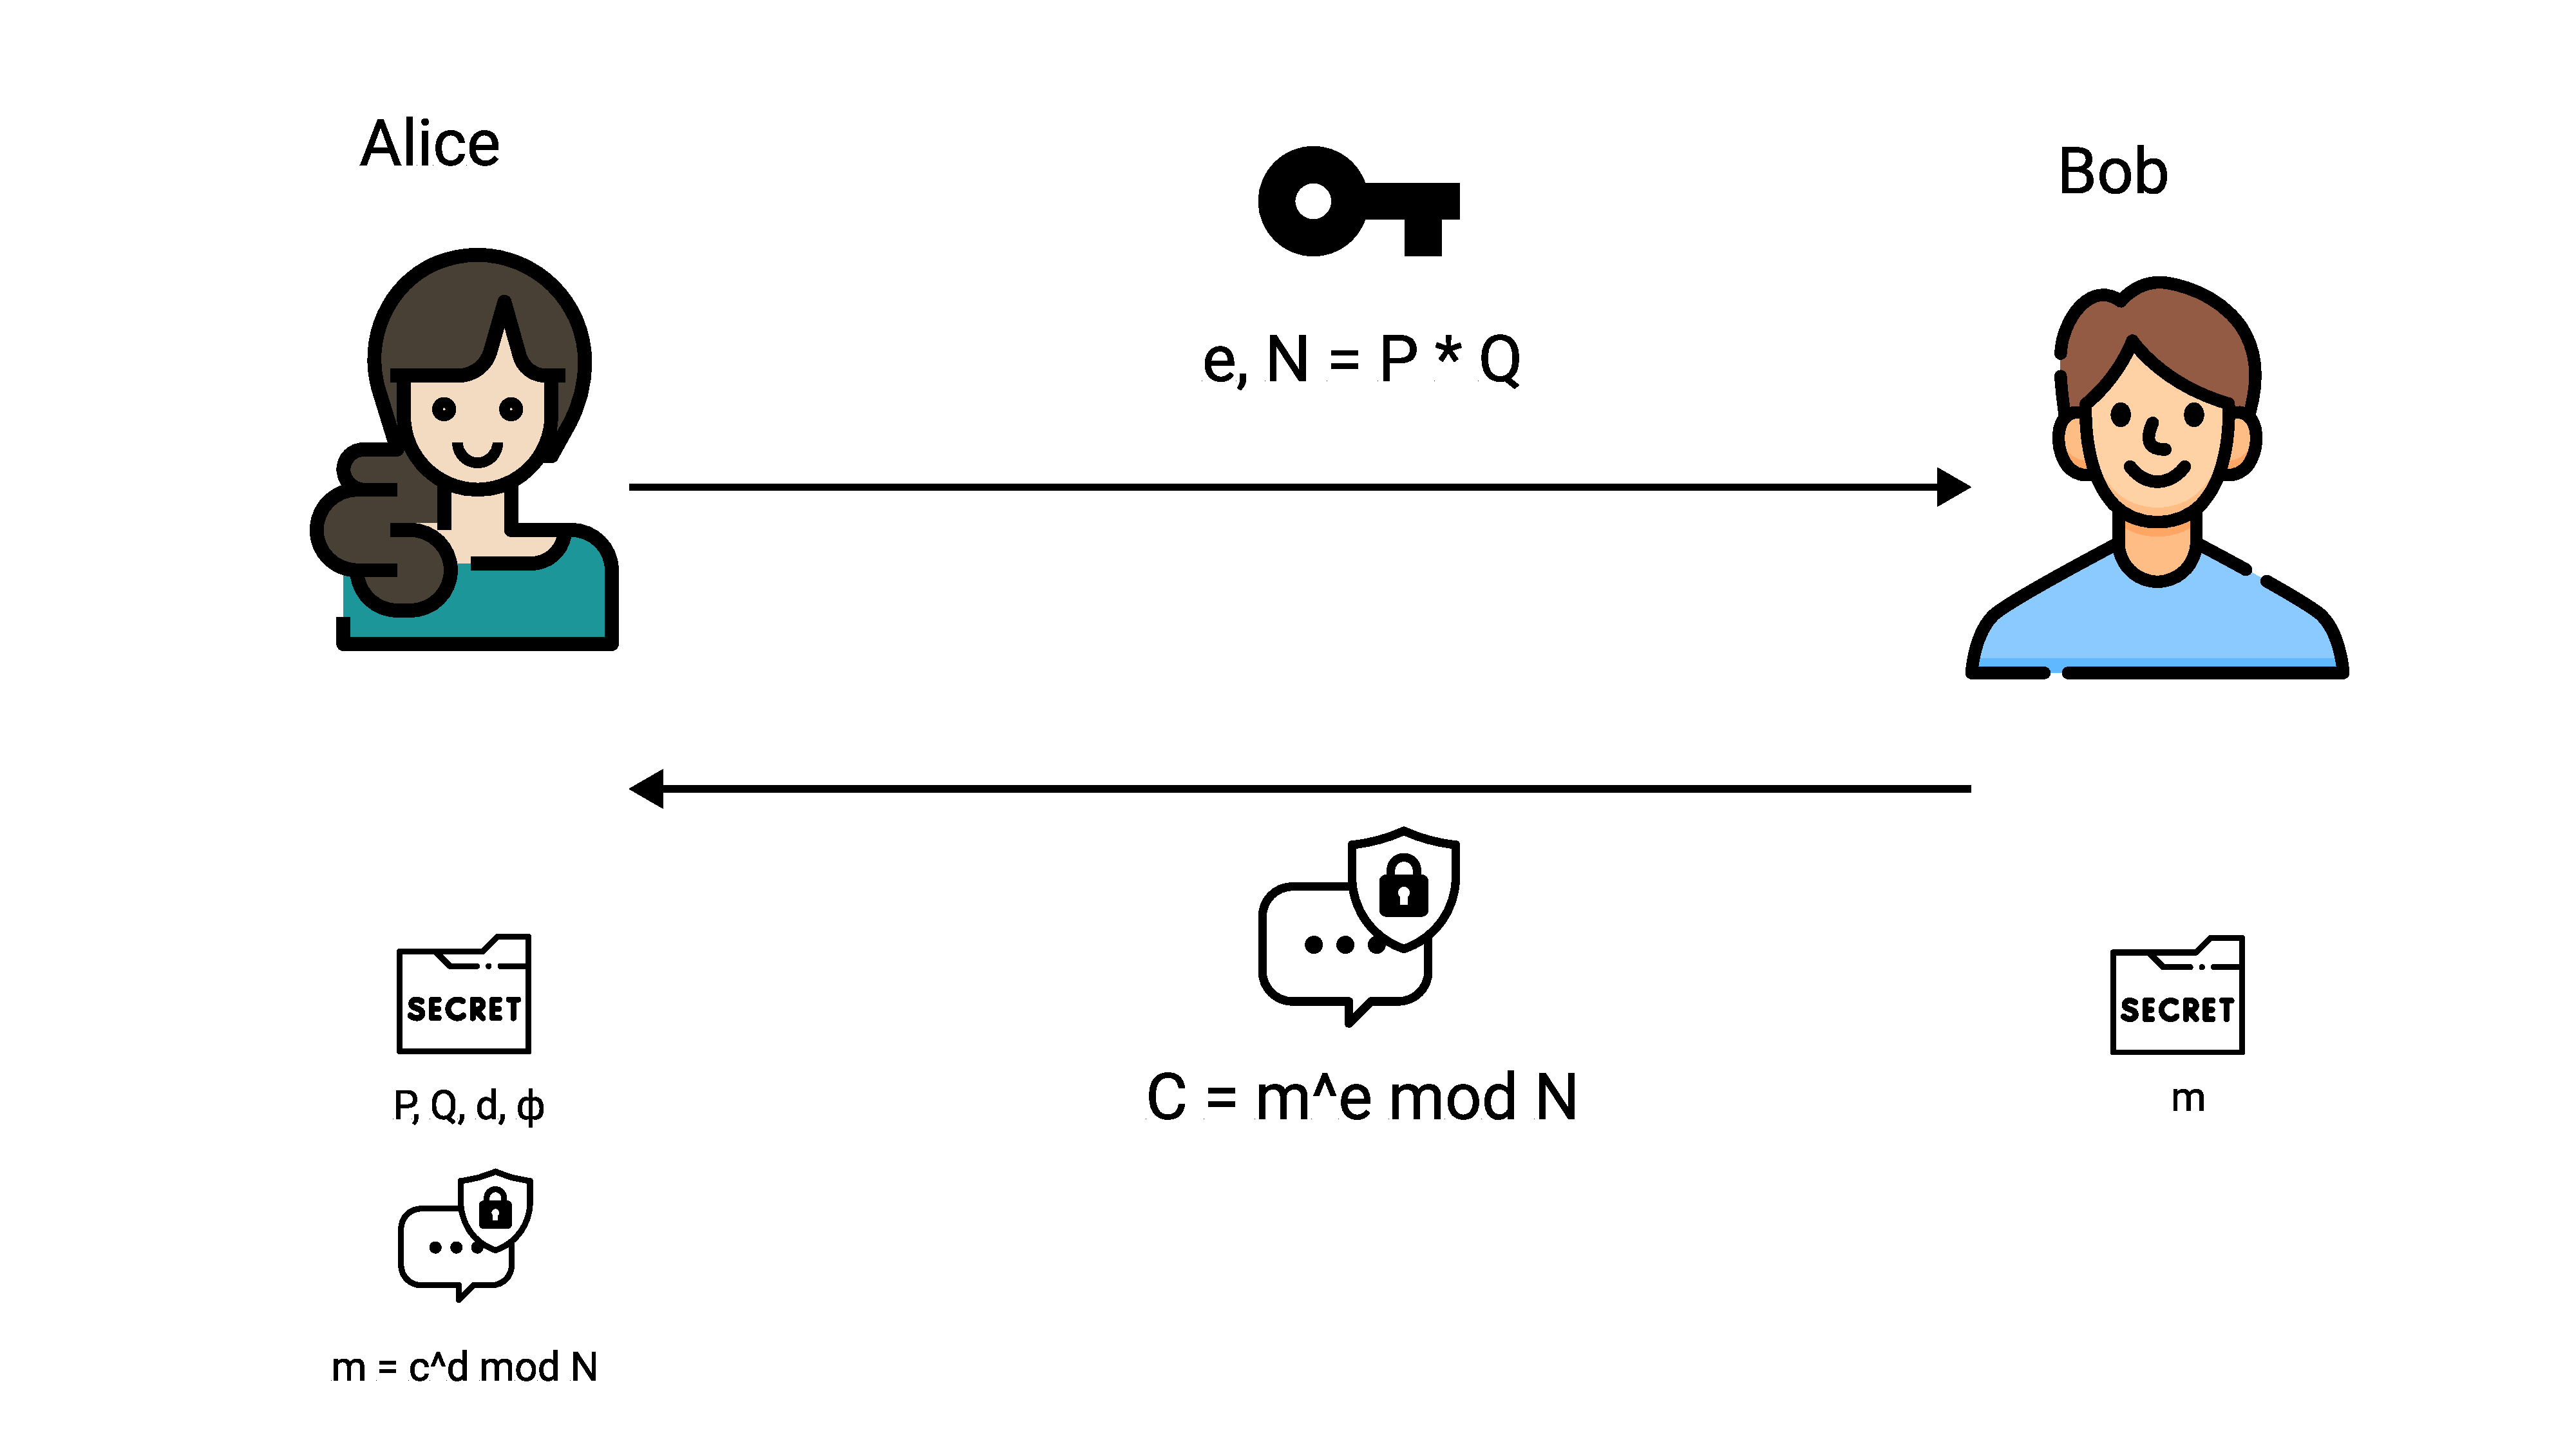
\includegraphics[width=1\textwidth]{./img/RSA}
    ~\caption{RSA algorithm concept diagram.}\label{fig:figure8}
\end{figure}
To summarize, the process by the steps is as follows
\begin{itemize}
    \item Alice defines the large secret prime numbers $P, \; Q$.
    \item Alice computes $N = P \cdot Q$ and $\phi = (P-1)(Q-1)$
    \item Alice chooses an integer $e$, $1<e< \phi$ such that $\gcd(e, \phi) = 1$.
    \item Alice computes secret exponent $d$, $1<d< \phi$ such that $ed \equiv 1 \bmod \phi$.
    \item Alice shares public key $(N,e)$ with Bob and keeps private key $(d, p, q)$ is secret.
    \item Bob defines the message $m$, encrypts it as $C = m^{e} \bmod N$.
    \item Bob sends $C$ to Alice.
    \item Alice decrypts $C$ using her secret $d$, so she gets $m$
    \[
        m = C^d \bmod N
    \]
\end{itemize}
Security of the RSA approach is based on the complexity of fundamental problem of prime factorization,
which takes decades to solve having enough large number.


    \bibliographystyle{unsrt}
    \bibliography{RSAEncryptionExplained}
    \noindent \textbf{Version:} \texttt{Local-0.1.0}

\end{document}
